\documentclass[11pt, fleqn]{amsart}
\usepackage{amsmath, amssymb, amsthm} 
\usepackage{hyperref}
\usepackage{mathtools}
\usepackage{graphicx}
\usepackage{adjustbox}
\usepackage{caption}
\usepackage{subcaption}
\usepackage{booktabs}
\usepackage{float}
\usepackage{longtable}
\usepackage{tikz-cd}
\usepackage{listings}
\usepackage{xcolor}
\newtheorem{theorem}{Theorem}[section]
\newtheorem{lemma}[theorem]{Lemma}
\newtheorem{corollary}[theorem]{Corollary}
\newtheorem{proposition}[theorem]{Proposition}
\newtheorem{observation}{Observation}
\theoremstyle{remark}
\newtheorem{remark}{Remark}
\DeclareMathOperator{\spec}{spec}
\title{From the sequence to the spectrum: the oscillation of $\mu_n$ for the
$h=2$ family, via Theorem~2.3}
\author{Barry Brent}
\email{axcjh@bu.edu}
\subjclass[2020]{05A17, 05C62, 11F11, 11P83}
\keywords{partitions, graphs, cusp forms}
\begin{document}
\maketitle
\vspace{-0.5em}
\begin{center}{14 June 2026}\end{center}
\vspace{1em}

This note carries the analysis of the constant sequence $h_0=1,\ h_n=2\ (n\ge1)$ one
step further than the two companion documents, which stopped at the coefficients $h_n$
(undeformed) and $h^{(c)}_n$ (deformed, with the limits $\cosh c,\sinh c$). Here we pass
all the way to the spectrum, i.e.\ to the minimum-modulus eigenvalue
$\mu_n=\min_{v\in E(\chi_n)}|v|$ of the matrix $J_{h,n}$, the quantity actually plotted in
the manuscript. As requested, we do \emph{not} go through the determinant/$\chi$
construction: we use Theorem~2.3 of the manuscript to pass directly from the sequence to
the characteristic polynomial, and then read the spectrum off the result.

The outcome is a complete and fully explicit account of the oscillation seen in
Figure~48B, including a correction to the unverified remark recorded there. In one
sentence: \emph{deformation by $c$ rigidly translates the entire eigenvalue cloud by $c$,
and the apparent oscillation of $\mu_n$ is nothing but the parity alternation of the
truncated $\cosh$ and $\sinh$ polynomials --- driven by exactly the same $(-1)^n$, coming
from the pole at $t=-1$, that splits the coefficients into $\cosh c$ and $\sinh c$.}

\section{The operator bridge}

We write $D=\dfrac{d}{dx}$ and recall that $\chi_n(x):=\chi\!\bigl(J_n(\overline{j})\bigr)(x)$
denotes the characteristic polynomial attached to the sequence $h$ through equation~(D).

\begin{proposition}\label{prop:bridge}
Let $H(t)=\sum_{r\ge0}h_r t^r$ be the generating function of the sequence. Then
\[
\chi_n(x)\;=\;H(-D)\,x^n ,
\]
the differential operator $H(-D)$ (a polynomial in $D$ when applied to $x^n$, since
$D^r x^n=0$ for $r>n$) applied to the monomial $x^n$.
\end{proposition}

\begin{proof}
Theorem~2.3 of the manuscript states
\[
\chi_n(x)=\sum_{r=0}^{n}\binom{n}{r}\,r!\,h_r\,(-1)^r\,x^{n-r}.
\]
Since $\binom{n}{r}r!=\dfrac{n!}{(n-r)!}$ and $D^r x^n=\dfrac{n!}{(n-r)!}\,x^{n-r}$, each
summand is $(-1)^r h_r\,D^r x^n$, so
$\chi_n(x)=\bigl(\sum_{r\ge0}h_r(-D)^r\bigr)x^n=H(-D)x^n$.
\end{proof}

Thus every structural feature of $H$ --- its poles, its residues, an exponential factor
--- becomes an operator acting on $x^n$, and the spectrum of $J_n$ is the zero set of the
resulting polynomial. Two facts about $H(-D)$ will do all the work: a simple pole of $H$
at $t=t_0$ contributes the operator $\dfrac{1}{1-t_0^{-1}(-D)}$-type resolvent
$\dfrac{\rho}{\,t_0-(-D)\,}$, and the entire factor $e^{ct}$ contributes $e^{-cD}$, which
is the translation operator $\bigl(e^{-cD}f\bigr)(x)=f(x-c)$.

\section{The deformed family: a rigid shift and a $\cosh/\sinh$ dichotomy}

For the deformed sequence $H^{(c)}(t)=e^{ct}/(1-t^2)$, Proposition~\ref{prop:bridge} and
the partial fraction $\dfrac{1}{1-t^2}=\tfrac12\bigl(\tfrac1{1-t}+\tfrac1{1+t}\bigr)$ give
\[
\chi^{(c)}_n(x)=H^{(c)}(-D)\,x^n
=e^{-cD}\,\frac{1}{1-D^2}\,x^n
=\Bigl(\tfrac{1}{1-D^2}\,y^n\Bigr)\Big|_{\,y=x-c}.
\]
Write $Q_n(y):=\dfrac{1}{1-D^2}\,y^n$, the polynomial solution of $Q_n-Q_n''=y^n$, namely
$Q_n=\sum_{k\ge0}D^{2k}y^n$.

\begin{lemma}\label{lem:Q}
\[
Q_n(y)=\tfrac{n!}{2}\bigl(E_n(y)+(-1)^nE_n(-y)\bigr)
=\begin{cases}
\displaystyle n!\!\!\sum_{0\le 2i\le n}\frac{y^{2i}}{(2i)!}, & n\ \text{even (a truncated }\cosh),\\[1.2em]
\displaystyle n!\!\!\sum_{0\le 2i+1\le n}\frac{y^{2i+1}}{(2i+1)!}, & n\ \text{odd (a truncated }\sinh),
\end{cases}
\]
where $E_n(z)=\sum_{m=0}^n z^m/m!$ is the $n$-th Taylor polynomial of $\exp$.
\end{lemma}

\begin{proof}
$\tfrac1{1-D}y^n=\sum_{k\ge0}D^k y^n=n!\sum_{m=0}^n y^m/m!=n!E_n(y)$, and likewise
$\tfrac1{1+D}y^n=(-1)^n n!E_n(-y)$. Average the two (the partial fraction). Finally
$E_n(y)+E_n(-y)$ retains the even powers and $E_n(y)-E_n(-y)$ the odd ones.
\end{proof}

\begin{corollary}[deformation is a rigid translation]\label{cor:shift}
$\chi^{(c)}_n(x)=Q_n(x-c)$, hence
\[
\spec\bigl(J^{(c)}_n\bigr)=c+\spec\bigl(J^{(0)}_n\bigr),
\qquad
\mu^{(c)}_n=\min_{Q_n(y)=0}|c+y| .
\]
The parameter $c$ translates the whole eigenvalue cloud by $c$ and changes nothing else.
\end{corollary}

\begin{theorem}\label{thm:limits}
Fix $c\in\mathbb{R}$. Then
\[
\lim_{\substack{n\to\infty\\ n\ \mathrm{even}}}\mu^{(c)}_n=\sqrt{c^2+\tfrac{\pi^2}{4}},
\qquad
\mu^{(c)}_n=|c|\ \text{ for every odd }n\ \text{(for all $n$ large enough this is the exact minimum).}
\]
\end{theorem}

\begin{proof}
By Lemma~\ref{lem:Q}, $\tfrac{1}{n!}Q_n(y)\to\cosh y$ (even $n$) and $\to\sinh y$ (odd
$n$), uniformly on compact sets, because the partial sums $E_n(\pm y)\to e^{\pm y}$ do. By
Hurwitz's theorem the zeros of $Q_n$ in any fixed disc converge to those of the limit
function; the remaining (``spurious'') zeros escape to infinity, their moduli growing
linearly in $n$. The zeros of $\cosh$ are $\pm i\pi(k+\tfrac12)$, the smallest being
$\pm i\pi/2$; the zeros of $\sinh$ are $\pm i\pi k$, namely $0$ and then $\pm i\pi,\dots$.

For even $n$ the smallest-modulus zeros of $Q_n$ approach $\pm i\pi/2$, so by
Corollary~\ref{cor:shift} the eigenvalue nearest the origin approaches $c\pm i\pi/2$ and
$\mu^{(c)}_n\to|c\pm i\pi/2|=\sqrt{c^2+\pi^2/4}$.

For odd $n$, $Q_n$ is an odd polynomial, so $y=0$ is a zero \emph{exactly}; hence $x=c$ is
an eigenvalue of $J^{(c)}_n$ for every odd $n$, giving $\mu^{(c)}_n\le|c|$. The remaining
zeros approach $\pm i\pi,\pm 2i\pi,\dots$ (moduli $\ge\pi$) together with the spurious
zeros (moduli $\to\infty$); once $n$ is large enough that all nonzero zeros $y$ satisfy
$|c+y|>|c|$, the minimum is attained at $y=0$ and $\mu^{(c)}_n=|c|$.
\end{proof}

\begin{remark}[the case $c=1$, and a correction to the manuscript]\label{rem:correction}
For $c=1$ the theorem gives $\mu^{(1)}_n=1$ on odd $n$ and
$\mu^{(1)}_n\to\sqrt{1+\pi^2/4}=1.86209588911\ldots$ on even $n$. High-precision
root-finding via Theorem~2.3 confirms this to many digits and shows the odd value is
$1$ \emph{exactly} for every odd $n$ in the computed range (see Figure~\ref{fig:mu},
left, and Figure~\ref{fig:cloud}).

This settles the unverified remark at Figure~48B. The even limit
$\sqrt{\pi^2/4+1}$ recorded there is correct. The companion statement that ``the heights
of the odd sequence really are exactly zero'' is \emph{not} correct: a height $\mu_n=0$
would require $0\in\spec(J^{(c)}_n)$, i.e.\ $\chi^{(c)}_n(0)=(-1)^n n!\,h^{(c)}_n=0$, i.e.\
$h^{(c)}_n=0$; but $h^{(c)}_n\to\sinh c=\sinh 1\neq0$ on odd $n$, so $0$ is never an
eigenvalue for large odd $n$. The correct odd height is the \emph{shifted origin}
$x=c$, of modulus $|c|=1$ --- exactly the ``apparently constant value one'' that the
manuscript reports from the plot.
\end{remark}

\begin{figure}[H]
\centering
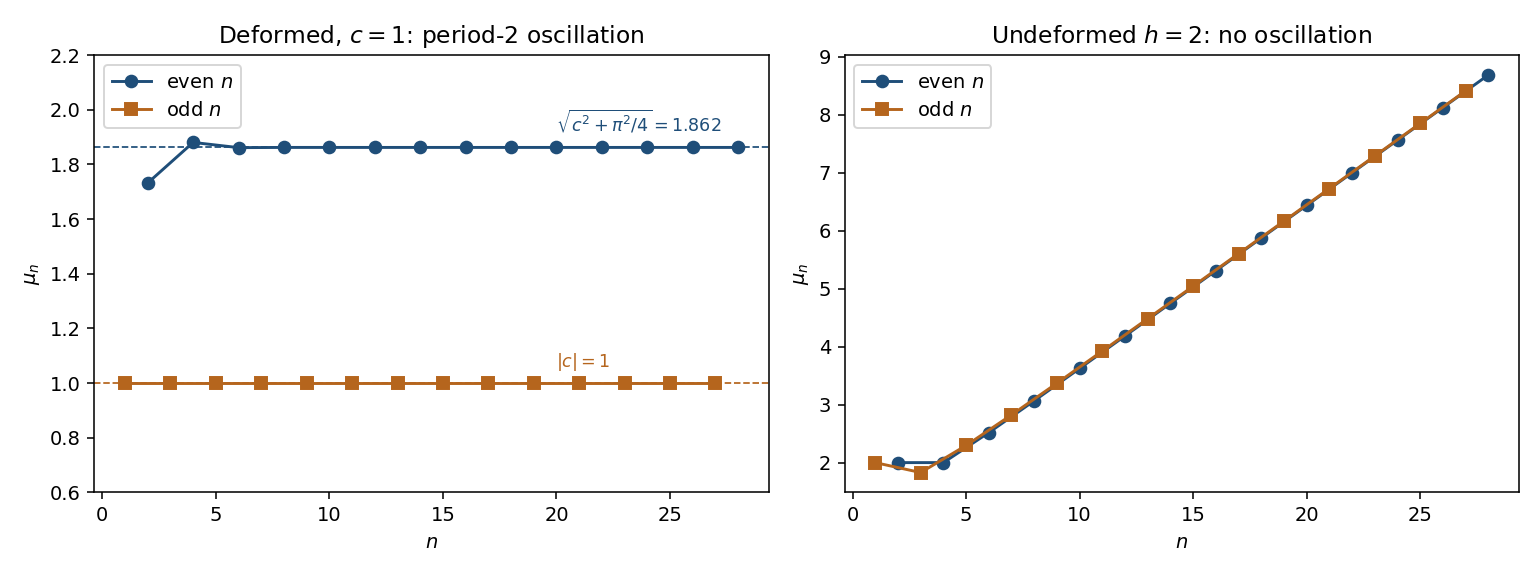
\includegraphics[width=\textwidth]{fig_mu.png}
\caption{Minimum-modulus eigenvalue $\mu_n$ computed from Theorem~2.3.
\emph{Left:} deformed $c=1$. Odd $n$ sit on $|c|=1$ (the eigenvalue $x=c$ forced by the
zero of the truncated $\sinh$); even $n$ climb to $\sqrt{c^2+\pi^2/4}=1.862$ (the shifted
zero $c\pm i\pi/2$ of the truncated $\cosh$). This period-$2$ split \emph{is} the
oscillation. \emph{Right:} undeformed $h=2$. The even and odd points lie on a single
smooth curve growing linearly --- no parity split, no oscillation.}
\label{fig:mu}
\end{figure}

\begin{figure}[H]
\centering
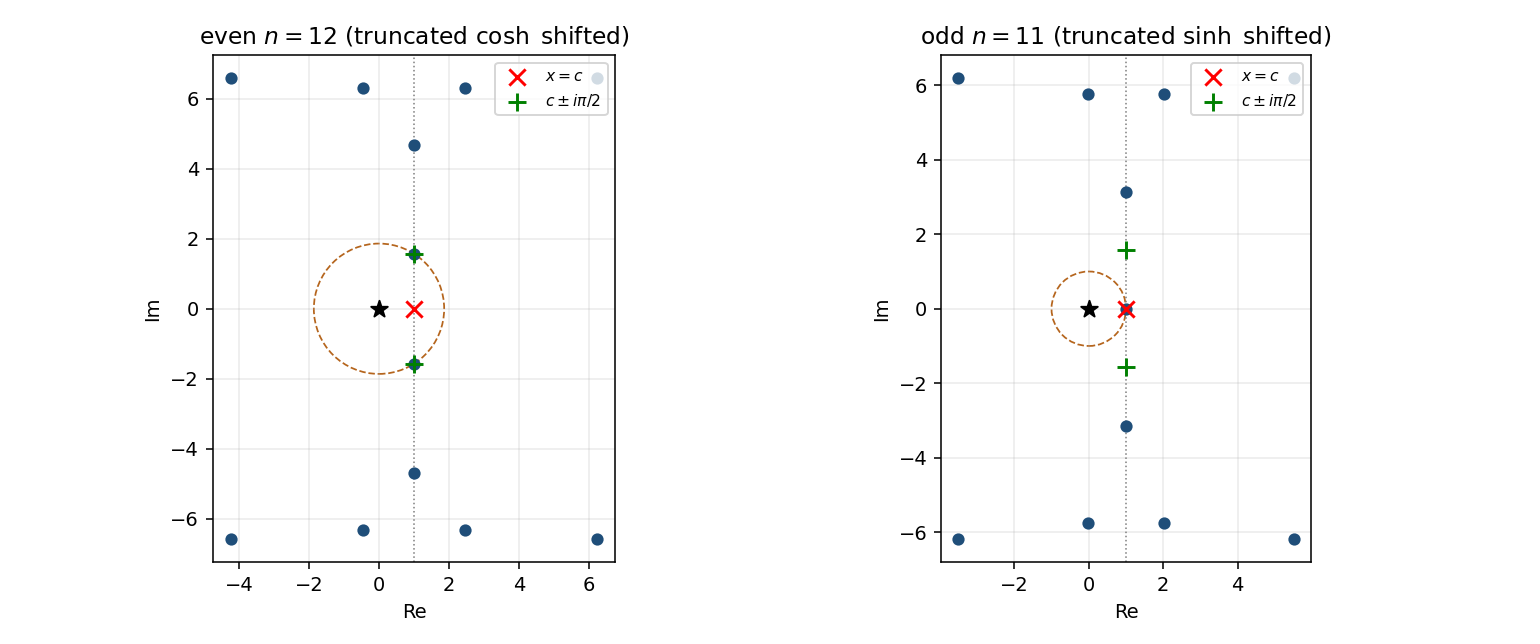
\includegraphics[width=\textwidth]{fig_cloud.png}
\caption{Eigenvalue clouds of $J^{(1)}_n$ in $\mathbb{C}$. By
Corollary~\ref{cor:shift} they are the zeros of a truncated $\cosh$ (even $n$, left) or
$\sinh$ (odd $n$, right), rigidly shifted to the line $\mathrm{Re}=c=1$ (dotted). The
star marks the origin and the dashed circle has radius $\mu_n$. \emph{Left:} the nearest
eigenvalues are $c\pm i\pi/2$ (green $+$). \emph{Right:} the truncated $\sinh$ vanishes at
$0$, so $x=c$ (red $\times$) is an eigenvalue and is the nearest one.}
\label{fig:cloud}
\end{figure}

\section{The undeformed sequence: one truncated exponential, no dichotomy}

For the undeformed sequence $H(t)=(1+t)/(1-t)$ the companion note records the
boundary decomposition $H(t)=\dfrac{2}{1-t}-1$: a single pole, at $t=+1$, with the pole at
$t=-1$ \emph{absent}. Proposition~\ref{prop:bridge} turns this directly into
\[
\chi_n(x)=H(-D)\,x^n=\Bigl(\tfrac{2}{1+D}-1\Bigr)x^n
=2(-1)^n n!\,E_n(-x)-x^n .
\]
The transcendental object controlling the zeros is now the truncated \emph{exponential}
$E_n(-x)$ --- the \emph{same} function for both parities; there is no $\cosh/\sinh$
alternation, because there is no second pole to supply the $\tfrac1{1-D}$ summand. The
correction $-x^n$ is negligible near the zeros of $E_n(-x)$: at such a zero $|x|$ grows
like $\kappa n$ (Szeg\H{o}: $x/n$ accumulates on the curve $|x\,e^{1-x}|=1,\ |x|\le1$,
with $\kappa\approx0.278$), and the ratio of the two terms is
$\sim(\kappa e)^{n}/(2\sqrt{2\pi n})\to0$. Hence the smallest-modulus eigenvalue grows
linearly, $\mu_n\sim\kappa n\to\infty$, as a single smooth (eventually increasing)
sequence with no even/odd split (Figure~\ref{fig:mu}, right). In particular $0$ is never
an eigenvalue, since $\chi_n(0)=(-1)^n\cdot 2\cdot n!\neq0$.

\section{What makes the difference}

\begin{remark}[the pole at $t=-1$ is the whole story, at the spectral level too]
Comparing the two computations, the oscillation of $\mu_n$ is governed by precisely one
feature of $H$: whether it has a second boundary pole, at $t=-1$.
\begin{itemize}
\item Under $t\mapsto -D$, a pole at $t=+1$ becomes the operator $\tfrac1{1+D}$ (truncated
exponential), and a pole at $t=-1$ becomes $\tfrac1{1-D}$. The deformed $1/(1-t^2)$ has
\emph{both}, with \emph{equal} residues, so they combine into the symmetric pair
$E_n(y)\pm E_n(-y)$ --- the truncated $\cosh$ and $\sinh$ of Lemma~\ref{lem:Q}. Their
alternation with the parity of $n$ is the spectral oscillation, and the alternating sign
is the very $(-1)^n$ that, at the coefficient level, splits $h^{(c)}_n$ into $\cosh c$ and
$\sinh c$.
\item The undeformed $(1+t)/(1-t)$ cancels the $t=-1$ pole with its numerator zero
(companion note, Lemma~2.1), leaving only $\tfrac1{1+D}$ --- one truncated exponential,
no alternation, no oscillation.
\end{itemize}
Thus the coefficient oscillation and the spectral oscillation are not two phenomena but
one, with a single cause (the pole at $t=-1$); Theorem~2.3, in the form
$\chi_n=H(-D)x^n$, is the exact conduit that carries that cause from the sequence to the
spectrum. A pair of boundary poles at $e^{\pm i\theta}$ would, by the same mechanism,
produce eigenvalues near $c\pm i\theta$-scaled directions and an oscillation of angular
frequency $\theta$; the case $\theta=\pi$ (poles at $\pm1$) is the period-$2$ even/odd
split seen here.
\end{remark}

\begin{remark}[scope]
Everything above is exact for the $h=2$ family, where $H$ is rational and $H(-D)$ is a
genuinely finite/resolvent operator. For the modular-form sequences that motivate the
manuscript the generating functions are not rational, the operator $H(-D)$ is not a finite
combination of resolvents, and locating the boundary singularities is itself the hard
problem; the present analysis does not claim to explain those cases. What it does provide
is a fully worked mechanism in the one family where every step is explicit, and a precise
template for the rest: find the dominant boundary singularities of $H$, and read the
oscillation --- in the coefficients and, through $\chi_n=H(-D)x^n$, in the spectrum ---
off their locations.
\end{remark}

\end{document}
